\section{iptables的使用}
\label{sec_iptables}


\begin{verbatim}
1.1)设定INPUT为ACCEPT 
    # iptables -P INPUT ACCEPT

1.2)设定OUTPUT为ACCEPT
    # iptables -P OUTPUT ACCEPT

1.3)设定FORWARD为ACCEPT
    # iptables -P FORWARD ACCEPT


2)定制源地址访问策略

2.1)接收来自192.168.0.3的IP访问
    # iptables -A INPUT -i eth0 -s 192.168.0.3 -j ACCPET

2.2)拒绝来自192.168.0.0/24网段的访问
    # iptables -A INPUT -i eth0 -s 192.168.0.0/24 -j DROP
 

3)目标地址192.168.0.3的访问给予记录,并查看/var/log/message
    # iptables -A INPUT -s 192.168.0.3 -j LOG


4)定制端口访问策略

4.1)拒绝任何地址访问本机的111端口
    # iptables -A INPUT -i eth0 -p tcp --dport 111 -j DROP

4.2)拒绝192.168.0.0/24网段的1024-65534的源端口访问SSH
    # iptables -A INPUT -i eth0 -p tcp -s 192.168.0.0/24 \
      --sport 1024:65534 --dport ssh -j DROP

5)定制CLIENT端的防火墙访问状态

5.1)清除所有已经存在的规则;
    # iptables -F

5.2)设定预设策略,除了INPUT设为DROP,其他为ACCEPT;
    # iptables -P INPUT DROP
    # iptables -P OUTPUT ACCEPT
    # iptables -P FORWARD ACCEPT

5.3)开放本机的lo可以自由访问;
    # iptables -A INPUT -i lo -j ACCEPT

5.4)设定有相关的封包状态可以进入本机;
    # iptables -A INPUT -i eth0 -m state \
      --state RELATED,ESTABLISHED -j ACCEPT
    # iptables -A INPUT -m state --state INVALID -j DROP


6)定制防火墙的MAC地址访问策略

6.1)清除所以已经存的规则
# iptables -F
# iptables -X
# iptables -Z

6.2)将INPUT设为DROP
# iptables -P INPUT DROP

6.3)将目标计算机的MAC设为ACCEPT
# iptables -A INPUT -m mac --mac-source \
  00-C0-9F-79-E1-8A -j ACCEPT

7)设定ICMP包,状态为8的被DROP掉
  # iptables -A INPUT -i eth0 -p icmp \
    --icmp-type 8 -j DROP

8)定制防火墙的NAT访问策略

8.1)清除所有策略
# iptables -F

8.2)重置ip_forward为1
# cat "1" > /proc/sys/net/ipv4/ip_forward

8.3)通过MASQUERADE设定来源于192.168.6.0网段的IP通过192.168.6.217转发出去
# iptables -t nat -A POSTROUTING -s 192.168.6.0 -o \
  192.168.6.217 -j MASQUERADE

8.4)通过iptables观察转发的数据包
# iptables -L -nv


9)定制防火墙的NAT访问策略

9.1)清除所有NAT策略
# iptables -F -t nat

9.2)重置ip_forward为1
# echo "1" > /proc/sys/net/ipv4/ip_forward

9.3)通过SNAT设定来源于192.168.6.0网段通过eth1转发出去
# iptables -t nat -A POSTROUTING -o eth1 \
  -j SNAT --to-souce 192.168.6.217

9.4)用iptables观察转发的数据包
# iptables -L -nv

10)端口转发访问策略

10.1)清除所有NAT策略
# iptables -F -t nat

10.2)通过DNAT设定为所有访问192.168.6.217的22端口,都访问到192.168.6.191的22端口
# iptables -t nat -A PREROUTING -d 192.168.6.217 \
  -p tcp --dport 22 -j DNAT --to-destination 192.168.6.191:22

10.3)设定所有到192.168.6.191的22端口的数据包都通过FORWARD转发
# iptables -A FORWARD -p tcp -d 192.168.6.191 --dport 22 -j ACCEPT

10.4)设定回应数据包,即通过NAT的POSTROUTING设定,使通讯正常
# iptables -t nat -I POSTROUTING -p tcp --dport 22 -j MASQUERADE

============================================================
# iptables -A INPUT -m state --state NEW -p tcp --dport 25 -j ACCEPT
# iptables -A INPUT -m state --state NEW -j DROP

修改目标地址在路由之前
# iptables -t nat -A PREROUTING -d 2.2.2.2 -p tcp \
  --dport 80 -j DNAT --to-destination 192.168.1.1:80

修改源地址在路由之后
# iptables -t nat -A POSTROUTING -s 192.168.1.0/24 \
  -o eth1 -j SNAT --to-source 1.1.1.1
\end{verbatim}

\subsection{内网机器通过iptables访问互联网}
\label{sec:InternalMachineInternet}

内网客户机通过一台Gnu/Linux服务器访问互联网。服务器的eth0网卡可以访问互
联网,服务器的eth1网卡与内网客户机相连。客户机通过该服务器访问互联网。

实验环境,

\begin{table}[!htbp]
  \centering
  \caption{iptables实验环境}
  \label{tab:iptables_test}
  \begin{tabular}{llll}
    \toprule
    角色 & IP & 网卡 & 网关 \\
    \midrule
    服务端 & 10.11.1.71/24 & eth0 & 10.11.1.1 \\
           & 192.168.56.109 & eth1 & 192.168.56.1 \\
    客户端 & 192.168.56.101 & eth0 & 192.168.56.109 \\
    \bottomrule
  \end{tabular}
\end{table}

实验环境已具备,接下来配置网关服务器。只需要简单的几步就可完成内网客户
机的上网需求。首先,开启服务器的内核转发功能,使其具备路由功能,设置如
下,

\begin{verbatim}
# echo 1 > /proc/sys/net/ipv4/ip_forward
\end{verbatim}

或则,

\begin{verbatim}
# sysctl -w net.ipv4.ip_forward=1
# sysctl -p
\end{verbatim}

设置完毕,可以在内网客户机上测试与服务器的连通性,

\begin{verbatim}
[root@client ~]# ping -c 2 192.168.56.109
PING 192.168.56.109 (192.168.56.109) 56(84) bytes of data.
64 bytes from 192.168.56.109: icmp_seq=1 ttl=64 time=5.76 ms
64 bytes from 192.168.56.109: icmp_seq=2 ttl=64 time=0.303 ms

--- 192.168.56.109 ping statistics ---
2 packets transmitted, 2 received, 0% packet loss, time 1002ms
rtt min/avg/max/mdev = 0.303/3.034/5.765/2.731 ms

[root@client ~]# ping -c 2 10.11.1.71
PING 10.11.1.71 (10.11.1.71) 56(84) bytes of data.
64 bytes from 10.11.1.71: icmp_seq=1 ttl=64 time=0.331 ms
64 bytes from 10.11.1.71: icmp_seq=2 ttl=64 time=0.331 ms

--- 10.11.1.71 ping statistics ---
2 packets transmitted, 2 received, 0% packet loss, time 999ms
rtt min/avg/max/mdev = 0.331/0.331/0.331/0.000 ms
\end{verbatim}


其次,配置NAT规则。由上一步骤的配置后,我们可以ping通服务器的各个网卡
的IP地址,但是内网主机还是无法访问互联网。内网机器需要通过地址转换后,
才能访问互联网。接下来配置NAT规则,

\begin{verbatim}
[root@server ~]# iptables -t nat -A POSTROUTING -s 192.168.56.0/24 \
> -o eth0 -j SNAT --to-source 10.11.1.71
[root@server ~]# iptables -A FORWARD -i eth1 -j ACCEPT
\end{verbatim}

\subsection{iptables之端口转发}
\label{sec:iptables_port_forward}

当我们的Web服务器在局域网内部,而且没有可在Internet上使用的真实IP地址,
那就可以使用DNAT让防火墙把所有到它自己HTTP端口的包转发给局域网内部真正
的Web服务器。目的地址可以是一个范围,这样的话,DNAT会为每一个流随机分配
一个地址。

注意,DNAT只能用在nat表的PREROUTING和OUTPUT链中,或者是被两条链调用的链
里。DNAT的选项为\verb|--to-destinatiion|,一个例子为,

\begin{verbatim}
# iptables -t nat -A PREROUTING -p tcp -d 116.236.245.210 \ 
--dport 22 -j DNAT --to-destinatiion 10.10.7.153-10.10.7.158
\end{verbatim}

解释:指定要写入IP头的地址,这也是包要被转发到的地方。上面的例子就是把
所有发往地址116.236.245.210的包都转发到一段局域网使用的私有地址中,
即10.10.7.153到10.10.7.158。如前所述,在这种情况下,每个连接都会被随机
分配到一个要转发到的地址,但同一个连接流总是使用同一个地址。我们可以只
指定一个IP地址作为参数,这样所有的包都被转发到同一台机器。我们还可以在
地址后指定一个或一个范围的端口。如:\verb|--to-destinatiion 10.10.7.158:80|或\verb|--to-destinatiion 10.10.7.158:80-100|。要注意,
只有先用\verb|--protocol|指定了TCP或UDP协议,才能使用端口。

下面来一个具体的例子,大致理解一下它是如何工作的。比如,我们想通
过Internet发布我们的网站,但是HTTP服务器在我们的内网里,而且我们对外只
有一个公有IP地址,就是防火墙那个对外的IP,即INET\_IP。防火墙还有一个内
网的IP,即LAN\_IP,HTTP的IP是HTTP\_IP(这也是内网地址)。为了完成我们设
想,要做的第一件事就是把下面的这个简单的规则加入到nat表中的PREROUTING链
中:

\begin{verbatim}
# iptables -t nat -A PREROUTING --dst INET_IP \ 
-p tcp --dport 80 -j DNAT --to-destinatiion HTTP_IP
\end{verbatim}

有了这条规则,所有从Internet来的并防火墙的80端口的数据包都会被转发到内
网的HTTP服务器上。下面是数据包

\begin{figure}[hbtp]
  \centering
  \caption{kvm桥接方式的网络拓扑}
  \label{fig:kvm_bridge_network}
  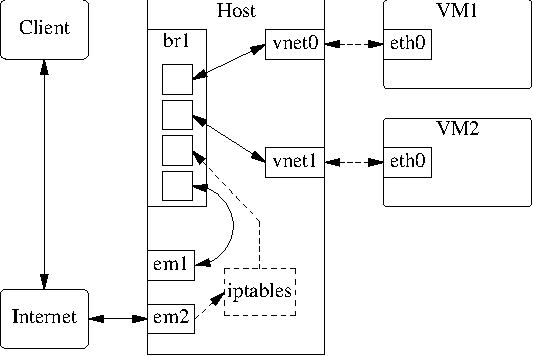
\includegraphics{graph/kvm_network.pdf}
\end{figure}
